\section{A -- Trapezoids}

\begin{frame}[fragile]{Problema}

You are given a trapezoid. The lengths of its upper base, lower base, and height are $a$, $b$, and 
$h$, respectively.

\begin{figure}
    \centering

    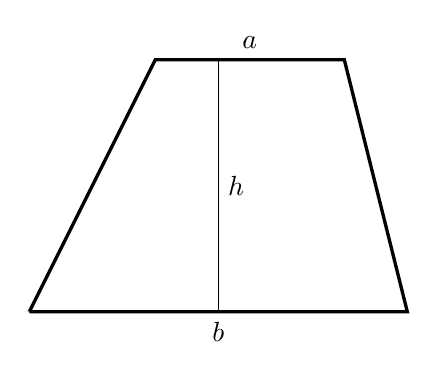
\begin{tikzpicture}[scale=0.8]
        \draw[very thick] (0, 0) -- (2, 4) -- node[anchor=south] { $a$ } (5, 4) -- (6, 0) --
            node[anchor=north] { $b$ } (0, 0);
        \draw (3, 0) -- node[anchor=west] { $h$ } (3, 4);
    \end{tikzpicture}
    \caption*{An example of a trapezoid}

\end{figure}

Find the area of this trapezoid.

\end{frame}

\begin{frame}[fragile]{Entrada e saída}

\textbf{Constraints}

\begin{itemize}
    \item $1\leq a\leq 100$
    \item $1\leq b\leq 100$
    \item $1\leq h\leq 100$
    \item All input values are integers.
    \item $h$ is even. 
\end{itemize}

\end{frame}

\begin{frame}[fragile]{Entrada e saída}

\textbf{Input}

Input is given from Standard Input in the following format:
\begin{atcoderio}{lll}
$a$ \\
$b$ \\
$h$ \\
\end{atcoderio}

\textbf{Output}

Print the area of the given trapezoid. It is guaranteed that the area is an integer.

\end{frame}

\begin{frame}[fragile]{Exemplo de entradas e saídas}

\begin{minipage}[t]{0.45\textwidth}
\textbf{Entrada}
\begin{verbatim}
3
4
2


4
4
4
\end{verbatim}
\end{minipage}
\begin{minipage}[t]{0.5\textwidth}
\textbf{Saída}
\begin{verbatim}
7




16
\end{verbatim}
\end{minipage}
\end{frame}

\begin{frame}[fragile]{Solução}

    \begin{itemize}
        \item O problema consiste na aplicação direta da fórmula da área do trapézio:
        \[
            A = \frac{(a + b)h}{2}
        \]
            
        \item Esta fórmula pode ser deduzida a partir da observação que o trapézio pode ser
            decomposto em um triângulo $T$ e um retângulo $R$

        \begin{figure}
            \centering

            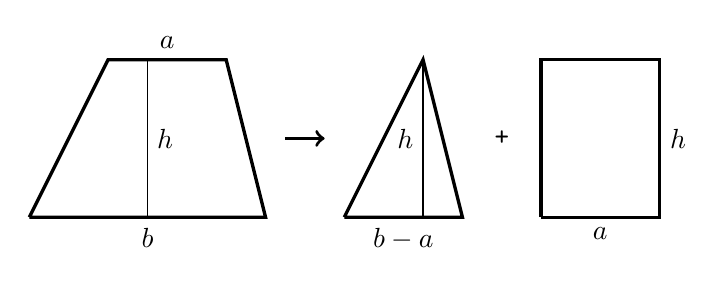
\begin{tikzpicture}[scale=0.5]
                \draw[very thick] (0, 0) -- (2, 4) -- node[anchor=south] { $a$ } (5, 4) -- (6, 0) --
                    node[anchor=north] { $b$ } (0, 0);
                \draw (3, 0) -- node[anchor=west] { $h$ } (3, 4);

                \draw[very thick] (8, 0) -- (10, 4) -- (11, 0) -- node[anchor=north] { $b - a$ } (8, 0);
                \draw (10, 0) -- node[anchor=east] { $ h $ } (10, 4);

                \draw[very thick] (13, 0) -- (13, 4) -- (16, 4) -- node[anchor=west] { $h$ } (16, 0) -- node[anchor=north] { $a$ } (13, 0);

                \draw[-latex,->,very thick] (6.5, 2) -- (7.5, 2);
                \node at (12, 2) { \texttt{\textbf{+}} };
            \end{tikzpicture}

        \end{figure}

    \end{itemize}

\end{frame}


\begin{frame}[fragile]{Solução}

    \begin{itemize}
        \item Assim,
        \begin{align*}
            A &= A_T + A_R \\
              &= \frac{(b - a)h}{2} + ah \\
              &= \frac{(a + b)h}{2}
        \end{align*}

        \item A aplicação direta da fórmula resulta em uma solução $O(1)$ para o problema
    \end{itemize}

\end{frame}
\begin{frame}[fragile]{Solução $O(1)$}
    \inputsnippet{cpp}{1}{21}{codes/A.cpp}
\end{frame}
